\chapter{Entwurf}
\section{Hardware}
Als Kamera wurde die AXIS M1031-M gewählt, da sie bereits gegeben war und den Anforderungen entspricht. Sie entspricht den oben genannten Anforderungen und hat den Vorteil einer einfachen Installation, welche aus Gründen der Irrelevanz hier nicht beschrieben wird.

\begin{figure}
\centering
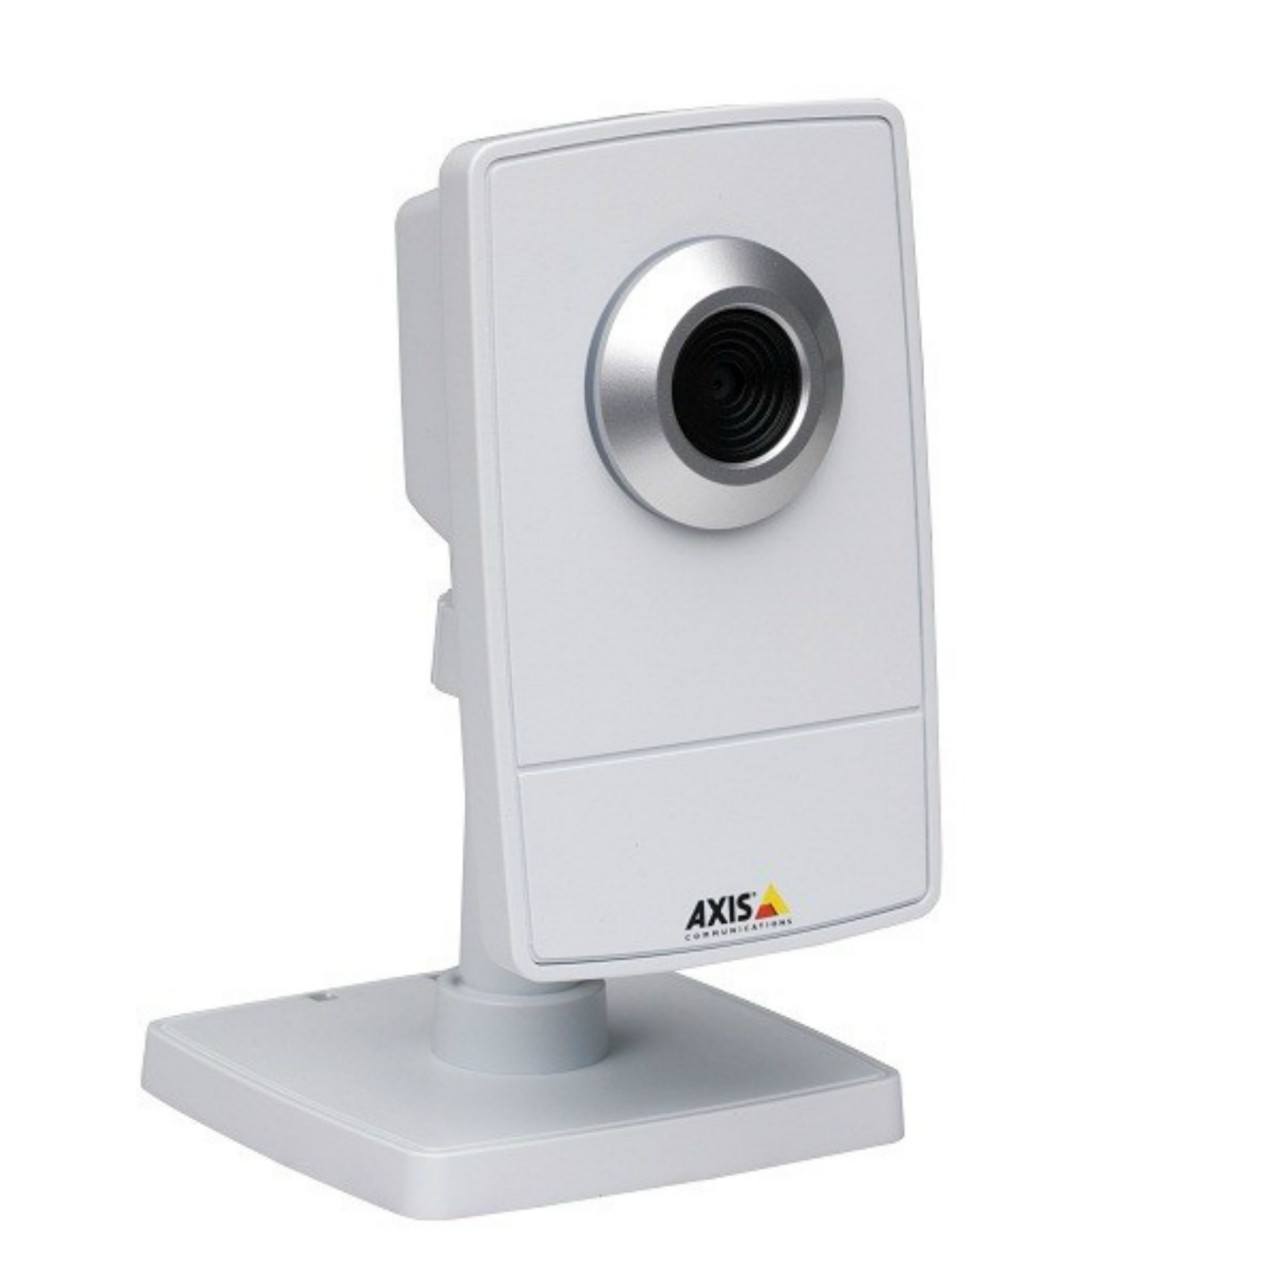
\includegraphics[width=.95\textwidth]{axis_camera} %{CS0031}
\caption[AXIS M1031-M]{AXIS M1031-M\footnotemark}
\label{fig:AXIS M1031-M}
\end{figure}
\footnotetext{\url{http://www.networkcamerastore.com/axis-m1031-w-0300-004-wireless-network-camera}}

\section{Software}
\begin{figure}
\centering
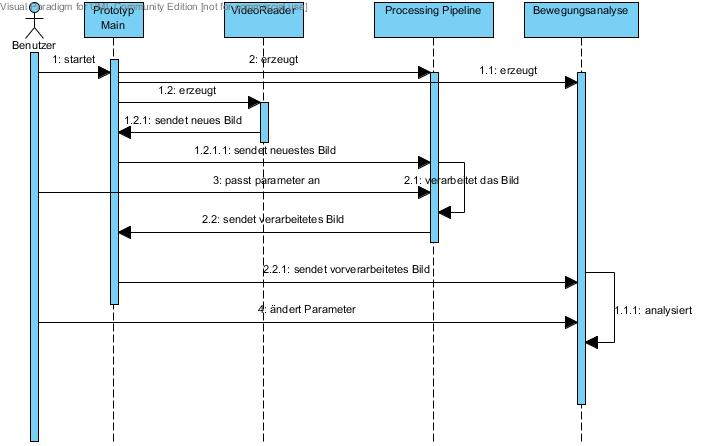
\includegraphics[width=.95\textwidth]{allgemeines_sequenzdiagramm} %{CS0031}
\caption[Allgemeines Sequenzdiagramm]{Allgemeines Sequenzdiagramm}
\label{fig:Allgemeines Sequenzdiagramm}
\end{figure}

\section{OpenCV}
\subsubsection{Installation}
Da die Geschwindigkeit des Programmes von Anfang an wichtig ist wurde sich dazu entschieden so viel arbeitslast wie möglich zu parallelisieren. Die Parallelsierung von Bildverarbeitsungsaufgaben bietet sich regelrecht an, da die Algorithmen wie folgt arbeiten: sie wenden die gleiche berechnung auf sehr viele zahlen/pixel an. Diese Arbeitsweise der Algorithmen ähnelt sehr stark der Arbeitsweise der GPU jeder Grafikkarte. 
Deswegen wurde sich dazu entschieden so viel wie möglich der Arbeitslast auf die GPU auzulagern, da zu beginn der Bearbeitung vermutet wurde, dass eine Sequenzielle bearbeitung der Berechnungen nicht ausreichen wird, da die Software in Echzeit Videodaten verarbeiten können soll.
OpenCV unterstützt seit der version 2.4.6. die benutzung der CUDA Runtime API und unterstützt ausschlie\ss{}lich NVIDIA GPU's. Um die GPU für OpenCV zu benutzen muss OpenCV eigenständig gebaut werden, die vorkompilierten versionen sind ohne CUDA support kompiliert. Dafür muss CUDA , die neuesten Grafikkartentreiber und eine NVIDIA Grafikkarte vorhanden sein. 
Die Kompilierung hat sich als etwas kompliziert herausgestellt, sodass die neueste version von \url{http://www.github.com/itseez/opencv}  mit dem tag 2.4.7. benutzt werden musste um eine erfolgreiche kompilierung abzuschlie\ss{}en. Dafür ist die Option WITH\_CUDA zu aktivieren, worauf man zusätzlich das Verzeichnis der NVIDIA CUDA installation angeben muss. Weiterhin habe ich OpenGL für die beschleunigte videodarstellung und OpenMP für die parallelisierung auf den CPUs aktiviert, um die die Grundbedingungen für die Geschwindigkeit der Software ausreichend zu erfüllen.
\subsubsection{Mat}
In OpenCV werden sämtliche Bilddaten als Matrizen abgebildet und der entsprechende Datentyp zur programmatischen Speicherung von Bilddaten heisst ensprechend Mat. Dieser Datentyp hält einige Informationen, wie die Grö\ss{}e des Bildes und der \emph{Typ} des Bildes. Die Grö\ss{}e beschreibt schlichtweg, wieviele Bildpunkte das Bild in der horizontalen, sowie in der vertikalen besitzt. Der Typ beschreibt, was für Bilddaten gespeichert sind. Wie bereits im Kapitel (??GRUNDLAGEN??) beschrieben können Bilder in unterschiedlichen Formaten, wie z.B. Grauwerte und Farbwerte gespeichert werden. OpenCV geht darüber hinaus und ermöglicht dem Entwickler zu bestimmen, wieviele \emph{channels} ein Bild hat und wie genau die Farbwerte gespeichert sind: \emph{depth}. Der Tabelle types können die diversen unterschiedlichen Typen entnommen werden.
\begin{table}
\caption[Mat Typen in OpenCV]{Mat Typen in OpenCV\footnotemark}
\label{tab:types}
\centering
\setlength{\tabcolsep}{5mm}	% separator between columns
\def\arraystretch{1.25}			% vertical stretch factor (Standard = 1.0)
\begin{tabular}{|r||c|c|c|c|} \hline
& \emph{C1} & \emph{C2} & \emph{C3} & \emph{C4}\\
\hline\hline
CV\_8U & 0 & 8 & 16 & 24\\
\hline
CV\_8S & 1 & 9 & 17 & 25\\
\hline
CV\_16U & 2 & 10 & 18 & 26\\
\hline
CV\_16S & 3 & 11 & 19 & 27\\
\hline
CV\_32S & 4 & 12 & 20 & 28\\
\hline
CV\_32F & 5 & 13 & 21 & 29\\
\hline
CV\_64F & 6 & 14 & 22 & 30\\
\hline
\end{tabular}
\end{table}
\footnotetext{\url{http://ninghang.blogspot.de/2012/11/list-of-mat-type-in-opencv.html}}
